%\documentclass[a4paper,12pt,final,twoside]{scrartcl}
\setcounter{secnumdepth}{3}
\setcounter{tocdepth}{5}

\usepackage[utf8]{inputenc}
\usepackage[T1]{fontenc}
\linespread{1.4}
\usepackage{dsfont}
\usepackage{amsfonts}
\usepackage{amsmath}
\usepackage{amssymb}
\usepackage{amsthm}
\usepackage{mathtools}
\usepackage{mathbbol}
\usepackage{amsmath1}
\usepackage[ngerman]{babel}
\usepackage{bibgerm}
\usepackage[pdftex]{graphicx}
%\usepackage{mathpazo}
\usepackage{floatflt}
%%\usepackage{epsfig}
\usepackage{wrapfig}
\usepackage{graphicx}
\usepackage{tabularx}
\usepackage{caption} 
\usepackage{multicol} 
\usepackage{mathrsfs}
%\usepackage{pspicture}
%\usepackage{eepic}
%\usepackage{epic}
%\usepackage{trfsigns}

%\usepackage[ansinew]{inputenc}
\usepackage{longtable,array,dcolumn}
%\usepackage{ngerman}
\usepackage{epic}
\usepackage{rotate}
\usepackage{graphpap}
\usepackage{amssymb}
\usepackage[squaren]{SIunits}
\usepackage{curves}
\usepackage{float}
\usepackage{array}
\usepackage{enumerate}
\usepackage{marvosym}
\usepackage{slashed}%für feynmanslsash
\usepackage[breaklinks,pdfborder={0 0 0}]{hyperref}
\usepackage{ulem}	%angeblich funktioniert dann
\let\underbar\uline	%underbar in math auch bei greek letters
\usepackage{multirow}
%\usepackage{multicolumn}
\usepackage{enumitem}


\setlength{\parskip}{12pt}
\setlength{\parindent}{0mm}
%\newcommand{\grad}{\ensuremath{^{\circ}}
%\renewcommand{\figurename}{Abb.}		% mit usepackage caption2
%\renewcommand{\captionfont}{\small \itshape}	% mit usepackage caption2
%\setkomafont{caption}{\small \itshape}		%sollte mit caption im userpackage funktionieren
%\setkomafont{captionlabel}{\small , \itshape}	%sollte mit caption im userpackage funktionieren
\captionsetup{font = {small, sf}} %mit it anstelle von sf gibts kusiv

\date{2009-20-10}
\newcommand{\kreis}[1]{
 \qbezier(-#1,0)(-#1,#1)(0,#1)
  \qbezier(0,#1)(#1,#1)(#1,0)
  \qbezier(#1,0)(#1,-#1)(0,-#1)
  \qbezier(0,-#1)(-#1,-#1)(-#1,0)}
\newcommand{\s}{\ \big| \ }
\newcommand{\lo}{\left <}
\newcommand{\ro}{\ri >}
\newcommand{\g}{&=&}

\newcommand{\ham}{\mathcal H}
\newcommand{\hil}{\mathscr H}
\newcommand{\fok}{\mathscr F}
\newcommand{\wh}{\widehat}
%\newcommand{\left}{\left}
\newcommand{\ri}{\right}
\newcommand{\Sp}{\text{Sp}}
\newcommand{\babsatz}{\par \begingroup \leftskip=2cm}
\newcommand{\eabsatz}{\par\endgroup}

\newcommand{\D}{\text{\itshape D}}
\newcommand{\Lr}{\mathcal L }%\textit{L}}
\newcommand{\rot}{\text{rot}}
\newcommand{\divergenz}{\text{div}}
\newcommand{\grad}{\text{grad}}
\newcommand{\grat}{${}^{\circ}$}
%\newcommand{\tanh}{\text{tanh}} already defined

\newcommand{\RM}[1]{\text{\MakeUppercase{\romannumeral #1}}}
\newcommand{\dell}{\partial}
\renewcommand{\div}{\operatorname{div}}
\newcommand{\I}{\dot{\text{\i\!\i}}}
\newcommand{\e}{\mathrm{e}}
\newcommand{\ket}[1]{\mid\!\!\!\,\,{#1}\rangle}
\newcommand{\bra}[1]{\langle{#1}\!\!\!\,\,\mid}
\newcommand{\braket}[2]{\langle{#1}\!\!\!\,\,\mid\!\!\!\,\,{#2}\rangle}
\newcommand{\bracket}[3]{\langle{#1}\!\!\!\,\,\mid\!\!\!\,\,{#2}\!\!\!\,\,\mid\!\!\!\,\,{#3}\rangle}
\newcommand{\1}{\mathds{1}}
\newcommand{\EW}[1]{\langle\!\!\,\,#1\!\!\,\,\rangle}
\newcommand{\arrowbox}[1]{-\!\!\!\!\:\text{(#1)}\!\!\!\;\;\!\!\!\rightarrow}

\newcommand{\ketI}[1]{\ket{#1}_{\!\!\;\text{I}}}
\newcommand{\ketII}[1]{\ket{#1}_{\!\!\;\text{II}}}
\newcommand{\ketIII}[1]{\ket{#1}_{\!\!\;\text{III}}}
\newcommand{\braI}[1]{\,\!_{\text{I}\!\!\;}\bra{#1}}
\newcommand{\braII}[1]{\,\!_{\text{II}\!\!\;}\bra{#1}}
\newcommand{\braketI}[2]{\,_{\text{I}\!\!\;}\braket{#1}{#2}_{\!\!\;\text{I}}\,}
\newcommand{\braketII}[2]{\,_{\text{II}\!\!\;}\braket{#1}{#2}_{\!\!\;\text{II}}\,}
\newcommand{\braketIII}[2]{\,_{\text{III}\!\!\;}\braket{#1}{#2}_{\!\!\;\text{III}}\,}
\newcommand{\bracketI}[3]{\,_{\text{I}\!\!\;}\bracket{#1}{#2}{#3}_{\!\!\;\text{I}}\,}
\newcommand{\bracketII}[3]{\,_{\text{II}\!\!\;}\bracket{#1}{#2}{#3}_{\!\!\;\text{II}}\,}


\newcommand{\up}{\ket{\uparrow}}
\newcommand{\updg}{\bra{\uparrow}}
\newcommand{\down}{\ket{\downarrow}}
\newcommand{\downdg}{\bra{\downarrow}}
\newcommand{\upup}{\ket{\uparrow\uparrow}}
\newcommand{\updown}{\ket{\uparrow\downarrow}}
\newcommand{\downup}{\ket{\downarrow\uparrow}}
\newcommand{\downdown}{\ket{\downarrow\downarrow}}

\newenvironment{itemize1}{\begin{itemize}[leftmargin=5mm,itemsep=-1ex,topsep=-1ex]}{\end{itemize}}

%\usepackage[left=2cm,right=2cm,top=1cm,bottom=1cm,includeheadfoot]{geometry}

\usepackage{fancyhdr}
\pagestyle{fancy}{\fancyhf{}
\fancyhead[LO,RE]{\footnotesize \rightmark}
\fancyfoot[C]{\footnotesize -$\,$\thepage$\;$-}
\renewcommand{\headrulewidth}{0.4pt}
\renewcommand{\footrulewidth}{0pt}}

\fancypagestyle{plain}{\fancyhf{}
\renewcommand{\headrulewidth}{0.4pt}
\fancyfoot[C]{\footnotesize -$\,$\thepage$\,$-}}

\usepackage{titlesec}
\titleformat{\section}[display]{\sffamily\bfseries\Huge\center}{Kapitel \thetitle:}{1ex}{}{}
\newcommand{\kapitel}[2]{$\;$\vspace{-1.5cm} \section[#1]{#2} \rule{17cm}{0.4pt}\vspace{3cm}}
\titleformat{\paragraph}[hang]{\sffamily\bfseries}{\thetitle:}{0ex}{\vspace{-0.15cm}}{\vspace{0.5cm}}

\title{ \vspace{1.5cm}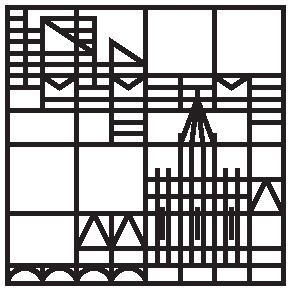
\includegraphics[width=5cm]{logo}
\\ \Large Universität Konstanz  \\ \vspace{4ex} \huge 
Skript zur Vorlesung\\ Höhere Quantentheorie und Elektrodynamik
\\ \vspace{4ex} \Large Prof. Dr. Wolfgang Belzig 
\\ Version vom 30. Juli 2012 \\ \vspace{4.5cm}
\normalsize Ursprünglichen Mitschrift von Birte Heinze im WS 09/10 \\ Ausführliche Überarbeitung von Tobias Lohse im WS 11/12 \vspace{-10cm}}
\author{}
\date{}
%\begin{document}

\setcounter{subsection}{-1}
\subsection{Wiederholung der Grundlagen der Quantenmechanik}
In diesem ersten Abschnitt sollen die wichtigsten Grundlagen der Quantenmechanik wiederholt werden. Diese Darstellung legt dabei weniger Wert auf Vollständigkeit als vielmehr darauf die Formeln und Definitionen zusammen zufassen, welche in den folgenden Abschnitten gebraucht werden. 

\subsubsection{Zustand eines Systems}

Der Zustand eines Systems ist die Gesamtheit der zur vollständigen Beschreibung des Systems minimal erforderlichen Informationen. 

In der analytischen Mechanik ist der Zustand eines Systems zum Zeitpunkt $t$ definiert als Vektor aus generalisierten Koordinaten $\vec{r}(t)$ und Impulsen $\vec{p}(t)$ des Systems zu diesem Zeitpunkt. Der Zustand zum Zeitpunkt $t$ ist also einem Vektor in einem reellen Vektorraum mit Dimension $2N+1$, wobei $N$ die Anzahl der generalisierten Koordinaten ist. Der Zustand im Laufe der Zeit kann als Trajektorie in diesem Vektorraum beschrieben werden. 

In der Quantenmechanik wird der Zustand des Systems zum Zeitpunkt $t$ hingegen als Wellenfunktion $\psi(\vec{r},t)$ in einem {\bf Hilbertraum} $\hil$ beschrieben. Die Dimension und Basis des Hilbertraums wird dabei durch die Randbedingungen des Systems festgelegt. 

Die Wellenfunktion kann in der algebraisch vorteilhaften {\bf Diracnotation} als sogenannter {\bf Ket-Vektor} $\ket{\psi(t)}$ dargestellt werden, die explizite Darstellung der Zeitabhängigkeit wird dabei meist weggelassen. Zu jedem Ket kann ein sogenannter {\bf Bra-Vektor} $\bra{\psi}$ im dualen Raum definiert werden, so dass $\braket{\psi}{\phi}$ das Skalarprodukt zwischen den beiden Kets $\ket{\psi}$ und $\ket{\phi}$ darstellt. Damit kann der Ket-Vektor in der Diracnotation dann wie folgt mit der Wellenfunktion in der {\bf Schrödingernotation} identifiziert werden: 
\begin{eqnarray*}
	\text{Diracnotation: $\ket{\psi(t)}$}\qquad \braket{\vec{r}}{\psi(t)} &=& \psi(\vec{r},t) \qquad\text{Schrödingernotation: $\psi(\vec{r},t)$} 
\end{eqnarray*}

\paragraph{Basis}
Jeder Hilbertraum $\hil$ besitzt eine {\bf orthonormale Basis} (ONB), das heißt eine Anzahl von linear unabängigen Vektoren $[\;(\ket{b_i})_i\;]=\hil$, die orthogonal zu einander und normiert sind: $\braket{b_i}{b_j}=\delta_{ij}$. Jeder Zustand im Hilbertraum lässt sich in einer solchen orthonormalen Basis entwickelnd. Im falle eines endlich dimensionalen Hilbertraums lässt sich dies schreiben als: 
\begin{eqnarray*}
	\ket{\psi} &=& \sum_{i} \underbrace{\braket{b_i}{\psi}}_{=c_i} \ket{b_i}
\end{eqnarray*}
Die Faktoren $c_i$ sind die {\bf Koordinaten} des Vektors $\ket{\psi}$ in der Basis $(\ket{b_i})_i$. In einer endlichen Basis lässt sich der Zustand somit als Spaltenvektor schreiben. Im Falle eines unendlich dimensionalen Hilbertraums, wir die Summe einfach durch ein integral über alle Basisvektoren ersetzt. 

\subsubsection{Wahrscheinlichkeitsinterpretation}

Im Gegensatz zur analytischen Mechanik legt der Zustand in der Quantenmechanik nicht den Ausgang jeglicher Messergebnisse fest, sondern wird als Wahrscheinlichkeit interpretiert. Die Wahrscheinlichkeit am System im Zustand $\ket{\psi}$ ein Teilchen am Ort $\vec{r}$ zur Zeit $t$ zu messen $p_{\vec{r}}(t)$ ist nach der {\bf Bornschen-Wahrscheinlichkeitsinterpretation} gegeben durch: 
\begin{eqnarray*}
	p_{\vec{r}}(t) &=& |\psi(\vec{r},t)|^2 = |\braket{\psi(t)}{\psi(t)}| 
\end{eqnarray*}
Der Zustand muss daher für alle Zeiten normiert werden: 
\begin{eqnarray*}
	|\braket{\psi(t)}{\psi(t)}| = \int \mathrm{d}^3r\; |\psi(\vec{r},t)| &\overset{!}=& 1
\end{eqnarray*}
Die Wahrscheinlichkeitsinterpretation kann für beliebige Messgrößen verallgemeinert werden. Die Wahrscheinlichkeit $p_{m}(t)$ das System im Zustands $\ket{m}$ zu finden ist dann gegeben durch: 
\begin{eqnarray*}
	p_m(t) &=& |\braket{m}{\psi(t)}|^2
\end{eqnarray*}

\subsubsection{Zeitentwicklung und Schrödingergleichung}

Die Zeitentwicklung des Zustandes wird durch die {\bf Schrödingergleichung} beschreiben: 
\begin{equation}
	\I \hbar\; \partial_t \ket{\psi(t)} = \hat{\ham}(\vec{r},t) \ket{\psi(t)}	\label{SG}
\end{equation}
Der {\bf Hamiltonoperator} $\hat{\ham}(\vec{r},t)$ kann mittels des Korrespondenzprinzips aus der Hamiltonfunktion der analytischen Mechanik hergeleitet werden, indem die Koordinaten $r_i$ und ihre konjugierten Impulse $p_i$ kanonisch quantisiert werden. Dies bedeutet, dass die Variablen $r_i$ und $p_i$ als Operatoren $\hat{r}_i$ und $\hat{p}_i$ interpretiert werden, welch die {\bf Vertauschungsrelation} $[\hat{r}_i,\hat{p}_i]=\delta_{ij}\I\hbar$ erfüllen. 

Für ein Teilchen im elektromagnetischen Feld mit Vektorpotential $\vec{ A}(\vec{r},t)$ und skalarem Potential $\phi(\vec{r},t)$ ergibt sich dann beispielsweise folgender Hamiltonoperator:
\begin{eqnarray*}
	\hat{\ham}(\vec{r},t) &=& \frac1{2m} \Big( \hat{\vec{p}} - q\hat{\vec{A}}(\hat{\vec{r}},t)\Big)^2 + q\hat{\phi}(\hat{\vec{r}},t)
\end{eqnarray*}
Das elektrische Feld $\vec{E}$ und das magnetische Feld $\vec{B}$ ergeben sich, ganz normal zu: 
\begin{eqnarray*}
	\vec{E} = -\nabla\phi - \partial_t\vec{A} &\qquad& \vec{B} = \nabla \times \vec{A}
\end{eqnarray*}
Die Ortsoperatoren $\hat{\vec{r}}$ und Implusoperatoren $\hat{\vec{p}}$ ergeben sich aus der kanonischen Vertauschungsrelation im Orts- bzw. Impulsraum wie folgt: 
\begin{eqnarray*}
	\text{Ortsraum:}\qquad \hat{\vec{p}} \;\psi(\vec{r}) &=& -\I\hbar \vec \nabla_{\vec{r}}\;\psi(\vec{r})
	\\
	\text{Impulsraum:}\qquad \hat{\vec{r}} \;\psi(\vec{p}) &=& +\I\hbar \vec \nabla_{\vec{p}}\;\psi(\vec{r})
\end{eqnarray*}

\paragraph{Stationäre Zustände}
Falls die Potentiale $\hat{\phi}$ und $\hat{\vec{A}}$ zeitunabhängig sind, lässt sich mit folgendem Lösungsansatz die Zeitabhängigkeit separieren und es ergibt sich die sogenannte {\bf stationäre Schrödingergleichung}: 
\begin{eqnarray}
	\psi(\vec{r},t) = \e^{-\I\frac{E t}{\hbar}} \cdot \psi(\vec{r}) &\overset{(\ref{SG})}{\Rightarrow}& E \psi(\vec{r}) = \hat{\ham}(\vec{r})\psi(\vec{r}) \label{statSG}
\end{eqnarray}
Die Lösung der Schrödingergleichung reduziert sich damit auf ein Eigenwertproblem. Damit ist die Energie des Systems nicht kontinuierlich, sondern kann nur bestimmte quantisierte Eigenwerte annehmen. 

\subsubsection{Observablen und Operatoren}

Eine Observable ist eine messbarer Parameter des Systems. In der Quantenmechanik werden Observablen nicht als Funktionen der Parameter des Systems geschrieben, sondern als lineare hermitesche Operatoren, welche auf die Zustände des Systems wirken und mittels derer die Wahrscheinlichkeit einer Messung am System bestimmt werden kann. Damit ein Operator eine reelle Messgröße repräsentieren kann muss er die Bedingung der Hermitizität erfüllen: $\hat{A}=\hat{A}^{\dagger}$. 

\paragraph{Spektrum}
Jeder hermitesche Operator $\hat{A}$ kann in einer orthonormalen Basis $(\ket{b_i})_i$ entwickelt werden. In einem endlich dimensionalen Hilbertraum lässt sich dies wie folgt darstellen: 
\begin{eqnarray*}
	\hat{A} &=& \sum_{i,j} \ket{b_i}\underbrace{\bracket{b_j}{\hat{A}}{b_i}}_{= A_{ij}}\bra{b_j} = \sum_{i,j} A_{ij} \ket{b_i}\bra{b_j}
\end{eqnarray*}
Die Faktoren $A_{ij}$ sind dann die Matrixelemente des Operators $\hat{A}$ in der Basis $(\ket{b_i})_i$ und der Operator kann somit als reellwertige Matrix geschrieben werden. In unendlich dimensionalen Hilberträumen muss die Summe durch ein Integral ersetzt werden. 

Für jede Observable lässt sich eine orthonormale Basis finden, in der diese Matrix nur diagonal Elemente hat. Diese Basis wird als Eigenbasis des Operators und die Diagonalenelemente als Spektrum des Operators bezeichnet. Die Darstellung des Operators in seiner Eigenbasis wird auch als {\bf Spektralform} $\hat{A}=\sum_{i}a_i\ket{a_i}\bra{a_i}$ bezeichnet. Ein Element des Spektrum $a_i$ wird auch als {\bf Eigenwert} und das zugehörige Element der Eigenbasis als {\bf Eigenzustand} $\ket{a_i}$ bezeichnet, da sie folgende Eigenwertgleichung erfüllen: 
\begin{eqnarray*}
	\hat{A}\ket{a_i} &=& a_i \ket{a_i}
\end{eqnarray*}
Man spricht davon, dass $a_i$ ein Eigenwert des Operators $\hat{A}$ zum Eigenzustand $\ket{a_i}$ ist. 


\paragraph{Erhaltungsgrößen}

Eine Observable $\hat{A}$ ist eine Erhaltungsgröße des Systems, das heißt eine zeitliche Konstante $\mathrm{d}\EW{\hat{A}}/\mathrm{d}t=0$, genau dann wenn sie mit dem Hamiltonoperator kommutiert, dass bedeutet der {\bf Kommutator} wird 0: $[\hat{\ham},\hat{A}]=\hat{\ham}\hat{A}-\hat{A}\hat{\ham}=0$. 


\subsubsection{Messprozess}

Der {\bf Erwartungswert} der Messung einer Observable $\hat{A}$ am System mit Zustand $\ket{\psi}$ ist gegeben durch: $\EW{\hat{A}}=\bracket{\psi}{\hat{A}}{\psi}$. Der Erwartungswert entspricht dabei dem theoretischen Mittelwert nach beliebig vielen Messungen. Das Ergebnis einer einzelnen Messung hingegen ist immer ein Eigenwert $a_i$ des Operators $\hat{A}$ mit zugehörigem Eigenzustand $\ket{a_i}$. Der Mittelwert selbst ist nicht notwendigerweise ein Eigenwert. Der Erwartungswert einer Observable hat in diesem Sinne keine physikalische, sondern lediglich eine statistische Realität. 

Die Wahrscheinlichkeit $p_{a_i}$ für die Messung des Eigenwerts $a_i$ mit Eigenzustand $\ket{a_i}$ ergibt sich nach der Bornschen-Wahrscheinlichkeitsinterpretation dann zu: $p_{a_i}=|\braket{a_i}{\psi}|^2$

Zwei Observablen $\hat{A}$ und $\hat{B}$ sind nur gleichzeitig messbar, wenn sie gemeinsame Eigenzustände besitzen, was der Falls ist, wenn sie miteinander kommutieren: $[\hat{A},\hat{B}]=0$. 

\paragraph{Projektionspostulat}

Das Projektionspostulat besagt, dass sich das System nach der Messung des einer Observablen im Eigenzustand des gemessenen Eigenwerts befindet: 
\begin{eqnarray*}
	\ket{\psi} \quad\arrowbox{Messung von $a_i$}\quad \ket{a_i}
\end{eqnarray*}
Der Zustand eines Systems wird also durch die Messung in den Eigenzustand projiziert und damit verändert. Dies wird auch als {\bf Kollaps der Wellenfunktion} bezeichnet. Durch die Messung wird der Zustand des Systems somit geändert. In der Quantenmechanik gibt es somit eine weitere Form der Zeitentwicklung mit folgenden Eigenschaften: 

\begin{itemize1}
	\item Die Projektion ist eine nicht unitäre, das heißt unumkehrbar, Zeitentwicklung. 
	\item Bei der Projektion gehen alle Informationen über den Zustand $\ket{\psi}$ vor der Messung verloren.
	\item Nach der Projektion befindet sich das System in einem reinen Zustand, eine wiederholte Messung ergibt somit immer erneut den zuvor gemessenen Eigenwert.
\end{itemize1}


\subsubsection{freies Teilchen}

Für den Fall, dass kein Potential vorhanden ist, $\hat{V}=0$, spricht man von einem freien Teilchen. Der Hamilton Operator ergibt sich dann zu: $\hat{\ham}=\hat{\vec{p}}/2m$. Der Impulsoperator kommutiert offensichtlich mit dem Hamiltonoperator, $[\hat{\ham},\hat{\vec{p}}\,]=0$, und ist somit erhalten. Die Eigenzustände sind somit {\bf ebene Wellen}, die im Ortsraum wie folgt geschrieben werden: 
\begin{eqnarray*}
	\psi_{\vec k}(\vec{r}) &=& C \cdot \e^{\I \vec{k}\vec{r}} \qquad \text{mit: } \hat{\vec{p}}\;\;\psi_{\vec k}(\vec r) = \underbrace{\hbar\vec{k}}_{=\vec{p}}\psi_{\vec k}(\vec r)
\end{eqnarray*}
Die Energie-Eigenwerte $E_{\vec{k}}$ des Hamiltonoperators ergeben sich somit zu: $E_{k}=\hbar^2k^2/2 m=\hbar\omega_k$. Damit ergibt sich die Zeitentwicklung des Zustandes zu: $\psi_{\vec{k}}(\vec{r},t) = C\cdot\e^{\I(\vec{k}\vec{r}-\omega_kt)}$. 

Die allgemeine Lösung ist eine Überlagerung dieser ebenen Wellen in einem Wellenpaket: 
\begin{eqnarray*}
	\psi(\vec{r},t) &=& \int \mathrm{d}^3k\; C(\vec{k})\cdot\e^{\I\big(\vec{k}\vec{r}-\omega(k)t\big)} \qquad\text{mit: }\omega(k) = \frac{E(k)}{\hbar} = \frac{\hbar k^2}{2m}
\end{eqnarray*}


\subsubsection{Harmonischer Oszillator}

Für ein quadratisches Potential: $\hat{V} = m/2\cdot\omega^2 \hat{x}^2$, ergibt sich der Hamilton Operator des harmonischen Oszillators zu:
\begin{eqnarray*}
\hat \ham = \frac{\hat{p}^2}{2m} + \frac12 m\omega^2 \hat{x}^2
\end{eqnarray*}
Zur Lösung der Schrödingergleichung des harmonischen Oszillators nach der sogenannte Dirac-Methode, führen wir zunächst einheitenlose Koordinaten $\hat{P}=\hat{p}\cdot\hbar\ell$ und $\hat{X}=\hat{x}/\ell$ ein, wobei $\ell=\sqrt{m\omega/\hbar}$ die sogenannte Oszillator-Länge ist. Damit lässt sich der Hamiltonoperator dann wie folgt schreiben: 
\begin{eqnarray*}
	\hat{\ham} = \frac{\hbar\omega}{2} (\hat{P}^2+\hat{X}^2) \quad\text{mit: } \hat{P}=\sqrt{\hbar m\omega}\cdot\hat{p}\text{,  }\hat{X}=\sqrt{\frac {\hbar}{m \omega}}\cdot\hat{x} \text{,  }[\hat{X}, \hat{P}]=\I
\end{eqnarray*}
Es können nun der sogenannte {\bf Aufsteigeoperator} $\hat{a}^{\dagger}$ und der sogenannte {\bf Absteigeoperator} $\hat{a}$ definiert werden:
\begin{eqnarray*}
	\hat{a}=\frac1{\sqrt{2}}\cdot(\hat{X}+\I\hat{P}) &\quad& \hat{a}^{\dagger} = \frac1{\sqrt2}\cdot(\hat{X}-\I \hat{P})
\end{eqnarray*}
Der Kommutator ergibt sich zu: $[\hat{a},\hat{a}^{\dagger}]=1$. Außerdem wird noch der sogenannte {\bf Anzahloperator} $\hat{n}=\hat{a}^{\dagger}\hat{a}$ definiert, so dass sich der Hamiltonoperator einfach schreiben lässt und man direkt sieht, dass die Eigenzustände des Hamiltonoperators mit Eigenenergy $E_n$ die Eigenzustände $\ket{n}$ des Anzahloperators sind:
\begin{eqnarray*}
	\hat{\ham}=\hbar\omega\cdot\Big(\hat{n}+\frac12\Big) &\Rightarrow& \hat{\ham}\ket{n}=\underbrace{\hbar\omega\Big(n+\frac12\Big)}_{=E_n}\ket{n}
\end{eqnarray*}
Es lässt sich zeigen, dass die Eigenwerte des Anzahloperators die natürlichen Zahlen $n\in\mathbb{N}$ sind. Somit sieht man, dass der Anzahloperator angibt, in der wievielten Anregungen $E_n$ des Oszillators sich das System befindet. Außerdem lässt sich nun zeigen, dass die Auf- und Absteigeoperatoren tatsächlich die Anregung um ein Niveau anheben, beziehungsweise absenken: 
\begin{eqnarray*}
	\hat{a}^{\dagger}\ket{n} = \sqrt{n+1}\ket{n+1} &\qquad&\hat{a}\ket{n} = \sqrt{n}\ket{n-1}
\end{eqnarray*}
Der harmonische Oszillator ist eines wichtigsten Modelle in der Quantenmechanik, welches vielseitige Anwendungen in der Modellbildung und verschiedenen Näherungen hat. 


\subsubsection{Zentralpotential und Drehimpulsoperator}

Ein weiteres wichtiges Modellsystem in der Quantenmechanik ist ein Zentralpotential $V(\vec{r})=V(r)$, in welchen - wie wir aus der klassischen Mechanik wissen - der Bahndrehimpuls erhalten ist. Ein typisches Beispiel für ein solches System ist das Wasserstoffatom. 

Der Bahndrehimpulsoperator $\hat{\vec{L}}$ kann ganz 'normal' als Kreuzprodukt aus Impulsoperator $\hat{\vec{p}}$ und Ortsoperator $\hat{\vec{r}}$ definiert werden: $\hat{\vec{L}}=\hat{\vec{r}} \times \hat{\vec{p}}$. Es lässt sich leicht zeigen, dass für ein Zentralpotential der Drehimpulsoperator mit dem Hamiltonoperator $\hat{\ham}(\hat{\vec{r}},\hat{\vec{p}})=\hat{\ham}(\hat{r},\hat{\vec{p}})$ kommutiert $[\hat{\vec{L}},\hat{\ham}]=0$, der Drehimpuls ist also auch in der Quantenmechanik eine Erhaltungsgröße. 


\paragraph{Eigenschaften von Drehimpulsoperatoren}
Das Konzept des Drehimpulses in der Quantenmechanik kann verallgemeinert werden. Der Drehimpulsoperator ist durch eine spezifische Algebra ausgezeichnet, die als {\bf Drehimpulsalgebra} bezeichnet und durch folgende Bedingung beschrieben wird: 
\begin{eqnarray}
	[\hat{L}_i, \hat{L}_j] = \I\hbar\sum_{k=1}^{3} \varepsilon_{ijk} \hat{L}_k &\quad\Leftrightarrow\quad& \hat{\vec{L}} \times \hat{\vec{L}} = \I\hbar \hat{\vec{L}}	\label{Drehimpulsalgebra}
\end{eqnarray}
Jeder Satz von drei Operatoren, für die die Drehimpulsalgebra (\ref{Drehimpulsalgebra}) gilt, wird als quantenmechanischer Drehimpuls behandelt. Ein wichtiges Beispiel für einen anderen solchen Operator in der Quantenmechanik ist der Spinoperator $\hat{\vec{S}}$. 

Ein Drehimpulsoperator $\hat{\vec{L}}=\sum_{i\in\{x,y,z\}}\hat{L}_i \vec{e}_i$ hat einige wichtige Eigenschaften, auf die im folgenden eingegangen werden soll: 
\begin{itemize1}
	\item Der Drehimpulsbetragsoperator, beziehungsweise sein Quadrat $\hat{L}^2=\sum_{i\in\{x,y,z\}}\hat{L}_i^2$ kommutiert mit jeder Komponente des Drehimpulsoperators: 
	\begin{eqnarray*}
		[\hat{L}^2,\hat{L}_i] &=& 0 \qquad\forall i\in\{x,y,z\}
	\end{eqnarray*}
	\item Das Spektrum des Drehimpulsoperators lässt sich in der orthonormalen Basis der $\ket{m,l}$ entwickeln, welche folgende Eigenwertgleichungen erfüllen: 
	\begin{eqnarray*}
		\hat{L}^2 \ket{m,l} = \hbar^2\cdot l(l+1) \ket{m,l} &\quad\land\quad& \hat{L}_z \ket{m,l} = \hbar m\ket{m,l}
	\end{eqnarray*}
	Aus der Algebra folgt $l\in\{n/2\;\big|\; n\in\mathbb{N}\}$ und $m\in\{-l+n\;\big|\; n\in\mathbb{N}\land n\leq 2l\}$. Die Eigenwerte $m$ und $l$ sind somit quantisiert und werden auch als Quantenzahlen bezeichnet. Für jeden Zustand $\ket{l}$ lassen sich somit $2l+1$ Eigenzustände von $\hat{L}_z$ finden, man spricht davon, dass $\ket{l}$ $2l+1$-fach entartet ist. 
	\item Für die diskreten Zustände $\ket{l,m}$ können die  {\bf Leiteroperatoren} $\hat{L}^{\pm} = \hat{L}_x \pm \I\hat{L}_y$ definiert werden. Aus der Drehimpulsalgebra lässt sich folgern, dass gilt: 
	\begin{eqnarray*}
		[\hat{L}_z,\hat{L}^{\pm}] = \pm\hbar\;\hat{L}^{\pm} &\quad\land\quad& [\hat{L}^+,\hat{L}^-] = 2\hbar\;\hat{L}_z
	\end{eqnarray*}
	Daraus und aus der Normierung folgt dann die Wirkung auf die Eigenzustände: 
	\begin{eqnarray*}
		\hat{L}^{\pm}\ket{l,m} = \hbar \underbrace{\sqrt{l(l+1)-m(m\pm1)}}_{=a_{l,m}^{\pm}}\ket{l,m\pm1}
	\end{eqnarray*}
	Wegen $\hat{L}^+\ket{l,l}=0$ und $\hat{L}^-\ket{l,-l}=0$ ist dann sofort ersichtlich, dass $\ket{l,l}$ der maximale Zustand und $\ket{l,-l}$ der minimaler Zustand des Systems ist. 
\end{itemize1}

Ein klassisches Beispiel für ein Zentralpotential ist das Wasserstoffatom, dessen quantisierte Atomorbitale sich aus den Eigenschaften des Bahndrehimpulsoperators erklären lassen. Der Bahndrehimpuls $\hat{\vec{L}}$ der Wasserstoff-Elektronen kann ganzzahlige Werte für $l$ annehmen. Die Eigenzustände des Bahdrehimpulses sind die Kugelflächenfunktionen. 

Neben dem Bahndrehimpuls spielt in der Quantenmechanik der Spin $\hat{\vec{S}}$ - auch Eigendrehimpuls genannt - eine wichtige Rolle, welcher ebenfalls die Drehimpulsalgebra erfüllt. Dieser kann halbzahlige Werte annehemen und ist eine Eigenschaft eines jeden Teilchens, welche sich mittels relativistischer Quantenmechanik (siehe Kapitel 4) erklären lässt. 

Der Gesamtdrehimpuls $\hat{\vec{J}}$ eines Teilchen ist die Summe aus Bahndrehimpuls und Spin: $\hat{\vec{J}} = \hat{\vec{L}} + \hat{\vec{S}}$. 


%\end{document}